% Scribe template is a combination of 16831 and 10725. Thanks to those TAs!
\documentclass[11pt]{article}
\usepackage{latexsym}
\usepackage{amsmath}
\usepackage{amssymb}
\usepackage{amsthm}
\usepackage{bm}
\usepackage{epsfig}
\usepackage[tight]{subfigure}
\usepackage{hyperref}
\usepackage{listings}


\newcommand{\handout}[5]{
  \noindent
  \begin{center}
  \framebox{
    \vbox{
      \hbox to 5.78in { {#1} \hfill #2 }
      \vspace{4mm}
      \hbox to 5.78in { {\Large \hfill #5  \hfill} }
      \vspace{2mm}
      \hbox to 5.78in { {\em #3 \hfill #4} }
    }
  }
  \end{center}
  \vspace*{4mm}
}

\newcommand{\lecture}[5]{\handout{#1}{#2}{#3}{#4}{#5}}

\newtheorem{theorem}{Theorem}
\newtheorem{corollary}[theorem]{Corollary}
\newtheorem{lemma}[theorem]{Lemma}
\newtheorem{observation}[theorem]{Observation}
\newtheorem{proposition}[theorem]{Proposition}
\newtheorem{definition}[theorem]{Definition}
\newtheorem{claim}[theorem]{Claim}
\newtheorem{fact}[theorem]{Fact}
\newtheorem{assumption}[theorem]{Assumption}

% 1-inch margins, from fullpage.sty by H.Partl, Version 2, Dec. 15, 1988.
\topmargin 0pt
\advance \topmargin by -\headheight
\advance \topmargin by -\headsep
\textheight 8.9in
\oddsidemargin 0pt
\evensidemargin \oddsidemargin
\marginparwidth 0.5in
\textwidth 6.5in

\parindent 0in
%\parskip 1.5ex
\renewcommand{\baselinestretch}{1.1}

\begin{document}
\newcommand{\defeq}[0]{\ensuremath{\stackrel{\triangle}{=}}}
\def\x{\mathbf{x}}
\def\w{\mathbf{w}}
\def\K{\mathbf{K}}
\lecture{{\bf 16-822}: Geometry-based Methods in Vision (F17) }{Released: Nov-15., Due: Dec 06}{Lecturer: Martial Hebert}{TA: Aayush Bansal}{Homework 4}


\section{Exploring 3D Reconstruction! (60 Points)}
In this part of the homework, we will explore 3D reconstruction. Especially, we will study a full pipeline of a typical 3D reconstruction system using Structure from Motion (SfM) and Stereo Matching. Slightly different from the previous homeworks, this time you do not implement everything from scratch. Instead, you will delve into one of the existing packages for this purpose (Here we use the {\em SFMedu} system from the computer vision group at Princeton University) by analyzing the results and modifying some steps of particular interest and importance. This is also a very good way to understand the material taught in the class.

\subsection{What you are supposed to do:}
You need to both implement and answer questions as follows:

\begin{figure}[h!]
\centering
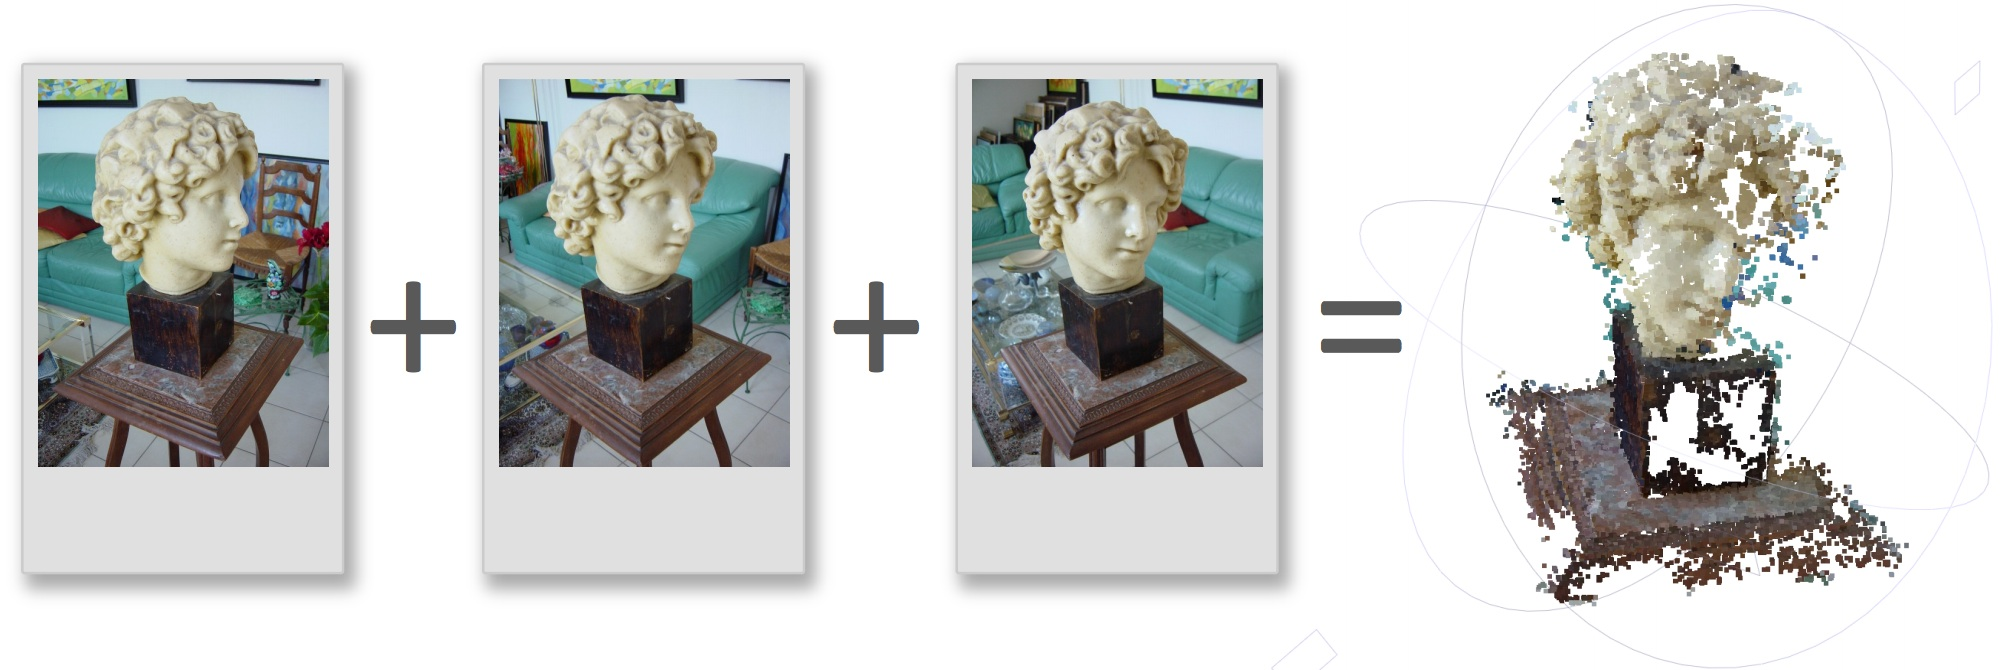
\includegraphics[width=0.9\textwidth]{tmpimages/teaser.jpg}
\caption{An illustration of the SFMedu system: Structure from Motion (SfM) and Stereo Reconstruction.}
\label{fig:sfmedu}
\end{figure}

\begin{itemize}
\item{{\bf{Run the SFMedu system}}\\
We have included the SFMedu package in $\texttt{./code/}$ folder. Run the SFMedu system by running the $\texttt{SFMedu2.m}$ script in MATLAB. Make sure that it runs successfully and produces a $\texttt{dense.ply}$ point cloud file. Install MeshLab from \url{http://meshlab.sourceforge.net}, and open the point cloud in MeshLab and rotate around the model. Take a screen capture of the point cloud and put it in the report as the answer to this question. An illustration is shown in Figure~\ref{fig:sfmedu}.}

\item{{\bf{List the Major Steps}}\\
Read the code carefully, especially $\texttt{SFMedu2.m}$. Summarize the major steps for SfM and dense stereo matching, and write it down in the report as answer to this questions.}

\item{{\bf{Principal Point}}\\
What is the assumption for the principal points in this system? Under what condition will this assumption get violated?}

\item{{\bf{Reconstruct Your Own Images}}\\
Capture/Find two sequences of images (at least $5$ images per set) on some interesting objects or scenes, run the system on these images. If it fails, figure out why it fails, and change the code or retake good images until it works. Submit the input images, as well as three screen captures of your reconstruction per image set in the report. Explain all the changes or things you have to do to make it work. Which step do you think is the most unstable one? Explain why. List suggestion for a normal user without any computer vision background about how to take good images to make it work.}

\item{{\bf{Compute the Reprojection Errors}}\\
Write a function\vspace{-0.05in}
$$\texttt{function printReprojectionError(graph)}\vspace{-0.05in}$$
that takes a graph (as defined in the SFMedu system), and prints out the current reprojection error, so that you can insert the function into many steps for debugging purpose, to check if the reconstruction errors are getting smaller. A call to this function is at Line 160 of $\texttt{SFMedu2.m}$. Submit the function as code. Also, plot the reprojection errors in the report for the image sequence provided and the two sets of images you captured in the report PDF file.}

\item{{\bf{Visualize the Reprojection Points}}\\
Write a function \vspace{-0.05in}
$$\texttt{function visualizeReprojection(graph,frames)}\vspace{-0.05in}$$
that takes a graph (as defined in the SFMedu system), and draw the 3D keypoint point cloud projected onto each image, as well
as their observed location. Figure~\ref{fig:visual} shows an example of the output for your function. You are required to write a function to produce the same kind of visualization. Each observed keypoint is represented by a red $\times$, and the reprojection of its 3D estimated location is represented by a green $+$, and these two points are connected by a blue line. For the 3D points that are projected to the image but not observed from the image, it should be shown as a yellow $\circ$. A call to this function is at Line 162 of $\texttt{SFMedu2.m}$. Submit the function as code, and also include the visualization results of the image sequence provided and the two sets of images you captured in the report PDF file.}

\begin{figure}[h!]
\centering
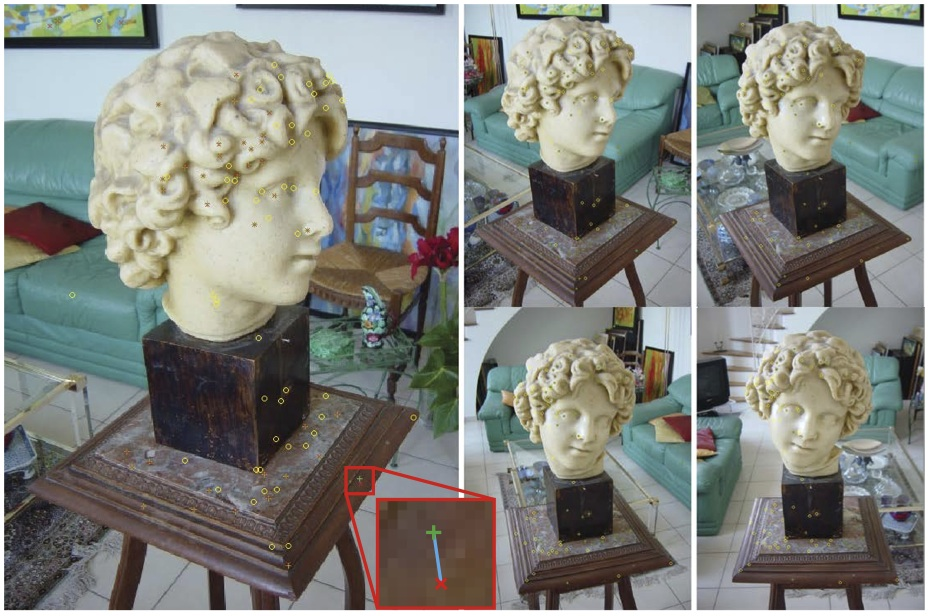
\includegraphics[width=0.95\textwidth]{tmpimages/visual.jpg}
\caption{An example result produced by \texttt{function visualizeReprojection(graph,frames)}.}
\label{fig:visual}
\end{figure}

\item{{\bf{Levenberg-Marquardt}}\\
$\texttt{bundleAdjustment.m}$ uses matlab function $\texttt{lsqnonlin}$ to minimize the objective function via the Levenberg-Marquardt algorithm: \vspace{-0.05in}
\begin{align*}
&\texttt{[vec,resnorm,residuals,exitflag] =}\\
&\texttt{lsqnonlin(@(x) reprojectionResidual(graph.ObsIdx,graph.ObsVal,px,py,f,x),}\\
&\texttt{[Mot(:);Str(:)], [], [], options);}
\end{align*}

Please read all the code and figure out what is the objective function it is optimizing for. Write down the math equation of this objective function in your report.

The Matlab implementation lsqnonlin of Levenberg-Marquardt is not suitable for very large scale problem. Read the document of lsqnonlin and explain why this statement is true in your report.}

\item{{\bf{Motion Adjustment Only}}\\
Bundle adjustment typically optimizes the Structure (the 3D location of the points) and the Motion (the camera parameters) together, as the above lines of code. But we can also fix the Structure, to adjust the Motion only, i.e., not allow the 3D points to move, but only changing the rotaiton and location of the cameras to optimize the objective function. With some good initialization, this can be used as a fine adjustment to solve camera resectioning task as well (\url{http://en.wikipedia.org/wiki/Camera_resectioning}). Fill in Line 34 in $\texttt{bundleAdjustment.m.}$

Please write down the math equation for the objective function, and also change the above line of code to do this. Submit the code and illustrate the results.}

\item{{\bf{Structure Adjustment Only}}\\
In the same way of thinking, we can also fix the Motion, to adjust Structure only, i.e., not allow the cameras to move, but only allows the 3D points to change their locations. Similarly, with some good initialization, this can be used as a fine adjustment to do ``triangulation'' for reconstructing the 3D point locations. Fill in Line 30 in $\texttt{bundleAdjustment.m}$.

Please write down the math equation for the objective function, and also change the above line of code to do this. Submit the code and illustrate the results.

Although this can be used to do triangulation, there is certain drawback. What is that? Answer this in the report.}


\item{{\bf{Smarter Graph Merging}}\\
The current reconstruction is merging the sequence sequentially, by adding one camera into the $\texttt{mergedGraph}$ in each step and do bundle adjustment again. A better graph merging will help to make the system more robust. For example, we can merge the graphs that have the maximal number of keypoint correspondences, instead of sequentially picking one. Change the code to implement a smarter graph merging. Submit the code and illustrate the results.}

\item{{\bf{Intrinsics}}\\
Change the code to optimize for the full intrinsics matrix. Submit the code and illustrate your results.}
\end{itemize}


\subsection{What you have to submit:}
\label{sec:tosubmit}
You should submit three files:
\begin{itemize}
\item A report that contains all the images (both the images you captured and your result images) and answers to the questions. (\textbf{25 Points})
\item Your \textbf{code} folder that contains all source code (including \textbf{your} readme) for your system, and your \textit{SFMedu2.m} script that takes no parameter as input and runs directly in Matlab to generate the results reported in your PDF file. (\textbf{25 Points})
\item Your \textbf{image} folder that contains all the input, intermediate and output images. (\textbf{10 Points})
\end{itemize}


\section{Geometric cues from Single Image (60 Points)}

Learning-based approaches have become popular to estimate geometric properties from single image. Here we will reason about the recent formulation for the problem of estimating depth and surface normal from single image. We will first explore how to formulate these problems, what are the problems with the current formulation, and how could we improve these formulation. 

\subsection{Depth estimation from a single image (40 Points)}
Estimating depth from a single image can be formulated as a regression problem, where you want to estimate the depth at each pixel. This problem has therefore largely been treated as a learning problem when a single image is provided. A lot of training data consisting of images and corresponding depth maps (obtained using Kinect or other 3D sensors) is used to train a model. At test time, this trained model is used to do inference over test images (generally not seen earlier, but roughly belonging to the same settings). This formulation however undermines the knowledge of geometry that we have learnt so far. In this section, our objective is to first understand this formulation, then figure out what is the problem with it, and finally propose new methods from our understanding in the geometry class that could potentially improve these approaches. Other than Hartley \& Zisserman book, you may want to check out the following papers to answer the questions in this section.
\begin{enumerate}
\item D. Eigen, and R. Fergus. \textit{Predicting Depth, Surface Normals and Semantic Labels with a Common Multi-Scale Convolutional Architecture}. In ICCV 2015. \url{https://cs.nyu.edu/~deigen/dnl/dnl_iccv15.pdf}.
\item I. Laina, C. Rupprecht, V. Belaigiannis, F. Tombari, and N. Navab. \textit{Deeper Depth Prediction with Fully Convolutional Residual Networks}. In 3DV 2016. \url{https://arxiv.org/pdf/1606.00373.pdf}.
\item A. Chakrabarti, J. Shao, and G. Shakhnarovich. \textit{Depth from single image by harmonizing overcomplete local network predictions}. In NIPS 2016. \url{http://www.cse.wustl.edu/~ayan/mdepth/}.
\end{enumerate}

Lets' take a \textbf{geometric} perspective of this problem. (\textbf{10 Points}).
\begin{enumerate}
\item Geometrically, what is wrong with the problem of single image depth estimation?
\item Reason  why we cannot get absolute depth from single image, and can only know the relative position in the scene.
\end{enumerate}

We will now explore the \textbf{formulation} of this problem. (\textbf{10 points})
\begin{enumerate}
\item As mentioned earlier, depth estimation from a single image can be formulated as a simple regression problem. Write mathematically the simplest formulation you could think of.
\item What are the problems with this formulation?
\item Propose a new formulation that could potentially overcome the above problems.
\item What are the problems that the proposed formulation can still not overcome, and why you think there is no way you could have incorporated required constraints in the above formulation to address these issues?
\end{enumerate}

Finally, about adding extra constraints from multiple cameras or motion cues; using the output reliably, and how to evaluate our formulation. (\textbf{20 points})
\begin{enumerate}
\item Suppose you have multiple views available, how will you modify the above formulation so that you can get the absolute scale? Recall that to get the depth from a stereo pair requires the knowledge of baseline.
\item Treating single image depth estimation as a regression problem can only provide the relative ``depth" values at test time. In class, Martial stressed the importance of knowing the confidence on the prediction/results so that it can be used reliably. Intuitively suggest how one could get the confidence scores from these systems OR how should one modify the current formulation to get the confidence score along with the predicted values.
\item What are the different criteria proposed in the literature to evaluate the output from a trained model? What is it that each one of these criterion can tell us about, and what it could not?
\end{enumerate}

\subsection{Surface normal estimation from a single image (20 Points)}
Somewhat similar is the formulation for estimating surface normal from a single image. You may want to check out the following papers to answer the question in this section. 

\begin{enumerate}
\item D. Fouhey, A. Gupta, and M. Hebert. \textit{Data-Driven 3D Primitives for Single Image Understanding}. In ICCV 2013. \url{https://people.eecs.berkeley.edu/~dfouhey/2013/3dp/index.html}
\item X. Wang, D. Fouhey, and A. Gupta. \textit{Designing Deep Networks for Surface Normal Estimation}. In CVPR 2015. \url{https://people.eecs.berkeley.edu/~dfouhey/2015/deep3d/deep3d.pdf}.
\item A. Bansal, B. Russell, and A. Gupta. \textit{Marr Revisited: 2D-3D Alignment via Surface Normal Prediction}. In CVPR 2016. \url{http://www.cs.cmu.edu/~aayushb/marrRevisited/}.
\end{enumerate}

Lets' formulate this problem, and see how can we improve the formulation with our understanding from the class. (\textbf{20 points})
\begin{enumerate}
\item Write a simple mathematical formulation for this problem?
\item What are the problems with this formulation?
\item Propose a new formulation that could potentially overcome the above problems.
\item Reason why you think the above formulation is sufficient to get reliable estimates. Is there something you think that could not be captured by your proposed formulation? Why you think it could not be incorporated in above formulation?
\item What are the different criteria proposed in the literature to evaluate the output from a trained model? What is it that each one of these criterion can tell us about, and what it could not?
\end{enumerate}

\noindent\textbf{One last word: } Feel free to drop an email to the TA in case you enjoyed working on this problem set (\textbf{Q2}), and you think that you want to experiment this formulation and see how it improves over state-of-the-art performance!


\end{document}
